% Compile using XeLaTeX (twice) or: tectonic -X compile main.tex
% This file and tables/*.tex are directly editable.
\documentclass[t,aspectratio=169,10pt]{beamer}
\usepackage{fontspec}
\usepackage{unicode-math}
\setmainfont{lmroman10-regular.otf}[BoldFont=lmroman10-bold.otf,ItalicFont=lmroman10-italic.otf,BoldItalicFont=lmroman10-bolditalic.otf]
\setsansfont{lmsans10-regular.otf}[BoldFont=lmsans10-bold.otf,ItalicFont=lmsans10-oblique.otf,BoldItalicFont=lmsans10-boldoblique.otf]
\setmonofont{lmmono10-regular.otf}
\setmathfont{latinmodern-math.otf}
\usepackage{amsmath,amssymb,graphicx,booktabs,array,csquotes}
\usepackage{tikz}
\usetikzlibrary{arrows.meta,positioning}
\def\slideContentLeftMargin{0.65cm}
\def\slideContentRightMargin{0.65cm}
\def\hustHeaderHeight{1.03cm}
\usepackage[blue,169]{beamerthemeHUST}
\graphicspath{{images/}{figures/}}
\HustShowPageNumtrue
\definecolor{accent}{HTML}{D55E00}
\definecolor{good}{HTML}{187A65}
\setbeamerfont{frametitle}{series=\bfseries,size=\large}
\setbeamerfont{caption}{size=\tiny}
\setbeamertemplate{caption}{\raggedright\insertcaption\par}
\setbeamercolor{block title}{fg=white,bg=hustprimary}
\setbeamercolor{block body}{bg=hustprimary!6}
\setbeamercolor{block title alerted}{fg=white,bg=accent}
\setbeamercolor{block body alerted}{bg=accent!7}
\setbeamercolor{block title example}{fg=white,bg=good}
\setbeamercolor{block body example}{bg=good!7}
\newcommand{\src}[1]{\par\vspace{3pt}{\tiny\color{black!55}Nguồn: #1\par}}
\newcommand{\notevi}[1]{\par\vspace{4pt}{\footnotesize #1\par}}
\newcommand{\hi}[1]{{\color{hustprimary}\bfseries #1}}
\newcommand{\warn}[1]{{\color{accent}\bfseries #1}}
\newcommand{\figslide}[3]{%
  \begin{frame}{#1}
    \begin{figure}\centering
      \includegraphics[width=\textwidth,height=4.75cm,keepaspectratio]{#2}
      \caption{#3}
    \end{figure}
  \end{frame}}

\title{Tổng hợp kết quả V10A và V10B}
\subtitle{Hiệu suất năng lượng, quỹ đạo UAV và vị trí BS}
\author{Báo cáo từ dữ liệu mô phỏng đã lưu}
\date{05/11/2026}

\begin{document}
% 1/10
\begin{frame}{V10A và V10B: tổng hợp kết quả}
\vspace{2mm}
{\Large\color{hustprimary}\bfseries EE, quỹ đạo UAV và vị trí BS}\par
\vspace{3mm}
\small Campaign 29/10/2026; báo cáo rút gọn ngày 05/11/2026.
\begin{block}{Ba kết quả chính}
\small Trong dữ liệu đã chạy:
\begin{itemize}
\item V10B tối ưu thêm Y; IPSO cho EE cao hơn A ở 21/21 cặp cấu hình, gain trung bình \hi{55,79\%}.
\item Sau loại trùng, IPSO đạt QoS ở \hi{42/42} tổ hợp A/B; Full PSO 41/42, JointPSO 24/42.
\item Tại $L=3$ Mbit, $q=5$ kbit, hover 1 s, cả \hi{12/12 nghiệm Full} đặt BS3 ở $(250,50,25)$ m.
\end{itemize}
\end{block}
\notevi{Phạm vi: 54 run, 216 kết quả; loại cấu hình lặp còn 42 run/168 kết quả. Ba seed: 2026, 608060, 3486784401. Cùng 120 particles, 1.000 vòng và một algorithm seed.}
\src{Campaign và 54 MAT đã đối chiếu trong bản đầy đủ; không chạy lại MATLAB/PSO.}
\end{frame}

% 2/10
\begin{frame}{Khác biệt A/B và vai trò của từng thuật toán}
\small
\begin{table}\centering
\begin{tabular}{p{3.0cm}p{5.0cm}p{5.0cm}}\toprule
Thành phần & V10A & V10B\\\midrule
Quỹ đạo & Tối ưu X; Y cách đều 15 m & Tối ưu X/Y; Y giảm ít nhất 1 m/đoạn\\
Hình học chung & \multicolumn{2}{l}{$Z=30$ m, 21 waypoint; $75\leq X\leq225$ m}\\
Đầu/cuối chung & \multicolumn{2}{l}{$(150,300,30)$ và $(150,0,30)$ m}\\
Số biến Joint/Full & 124/130 & 143/149\\\bottomrule
\end{tabular}\caption{B mở thêm tự do bố trí điểm phục vụ theo Y; mô hình kênh và năng lượng giống A.}
\end{table}
\footnotesize
\begin{description}
\item[JointPSO] Tối ưu quỹ đạo và alpha, giữ BS cố định.
\item[Full PSO] Thêm tối ưu X/Y của ba BS, rồi polishing alpha.
\item[IPSO] Cùng biến với Full PSO; giảm trọng số quán tính, thêm mutation và elite, rồi polishing.
\item[Baseline] Bay thẳng, BS cố định, alpha theo kênh; chỉ 2/42 tổ hợp khả thi nên chỉ dùng tham chiếu.
\end{description}
\src{Mã hình học, ba optimizer và cấu hình lưu trong MAT. IPSO là Full IPSO trong dữ liệu.}
\end{frame}

% 3/10
\begin{frame}{V10 lấy gì từ bài Drones và bổ sung những gì?}
\footnotesize
\begin{table}\centering
\begin{tabular}{p{2.5cm}p{5.1cm}p{5.4cm}}\toprule
Thành phần & Kế thừa từ Drones [1] & Triển khai trong V10A/V10B\\\midrule
Propulsion & Eq. (10)--(11), Table 2, bốn rotor & Profile + induced + parasite; cùng bộ hệ số\\
Lịch bay & Bay ngang, cùng tốc độ, phục vụ khi hover & $v=15{,}521$ m/s; thời gian bay $d_n/v$\\
Năng lượng & Năng lượng bay và RF; budget 17 kJ & Bổ sung riêng tải động cơ hover $P_f(0)\sum h_n$\\
Bài toán & Sum-throughput, BackCom, KKT/GSS, TSP/GA & Giữ SWIPT--NOMA và PSO/IPSO của dự án; tối đa bit/J\\\bottomrule
\end{tabular}\caption{V10 kế thừa nền vật lý, đồng thời điều chỉnh mục tiêu, giao thức và hạch toán hover.}
\end{table}
\[
\mathrm{EE}=\frac{\sum_{u,n}D_{u,n}}{P_f(v)\sum_n d_n/v+P_f(0)\sum_n h_n+E_{\rm RF}},\quad
\sum_nD_{u,n}\geq L,\quad D_{u,n}\geq q.
\]
\notevi{20 lần phục vụ: EH/UL trong $h/2$, RF/DL trong $h/2$, rồi bay. Cruise 108,9408 W; hover 172,3876 W. EH chỉ cấp RF lý tưởng. Tổng tải không vượt 17.000 J.}
\src{[1], Eq. (10)--(12), Table 2, tr. 8--9; cấu hình mô phỏng tr. 17. $L$: bit/user/nhiệm vụ; $q$: bit/user/slot.}
\end{frame}

% 4/10
\begin{frame}{EE theo L: Full PSO/IPSO đạt đủ ba seed}
\small\begin{table}
\centering
\renewcommand{\arraystretch}{1.16}
\setlength{\tabcolsep}{5pt}
\begin{tabular}{lrrrr}
\toprule
Bản & $L$ (Mbit) & JointPSO & Full PSO & IPSO \\
\midrule
V10A & 1 & 2\,236.1 (3/3) & 6\,041.6 (3/3) & 6\,082.9 (3/3) \\
V10A & 2 & 2\,418.8 (1/3) & 5\,624.1 (3/3) & 5\,857.0 (3/3) \\
V10A & 3 & -- (0/3) & 5\,420.5 (3/3) & 5\,649.7 (3/3) \\
V10B & 1 & 3\,438.0 (3/3) & 8\,721.0 (3/3) & 8\,343.6 (3/3) \\
V10B & 2 & 2\,549.2 (2/3) & 7\,157.0 (3/3) & 9\,360.2 (3/3) \\
V10B & 3 & 1\,876.0 (1/3) & 7\,556.7 (3/3) & 9\,390.4 (3/3) \\
\bottomrule
\end{tabular}
\caption{EE trung bình (bit/J) trên các seed khả thi. Số trong ngoặc: nghiệm khả thi/3.}
\end{table}

\notevi{Giữ $q=5$ kbit/user/slot, hover 1 s. JointPSO A giảm từ 3/3 xuống 0/3 nghiệm khả thi khi tăng $L$ từ 1 lên 3 Mbit.}
\notevi{EE của IPSO B tăng từ 8.343,6 lên 9.390,4 bit/J trong các nghiệm tìm được. Điều này phản ánh đường tìm kiếm hữu hạn; siết riêng $L$ không làm tối ưu toàn cục tăng.}
\src{Sweep $L$; Full PSO/IPSO sau polishing. Trung bình chỉ lấy seed khả thi, số trong ngoặc là n/3.}
\end{frame}

% 5/10
\begin{frame}{EE theo q: QoS từng slot có chi phí EE}
\small\begin{table}
\centering
\renewcommand{\arraystretch}{1.16}
\setlength{\tabcolsep}{5pt}
\begin{tabular}{lrrrr}
\toprule
Bản & $q$ (kbit) & JointPSO & Full PSO & IPSO \\
\midrule
V10A & 0 & -- (0/3) & 4\,417.0 (3/3) & 5\,500.2 (3/3) \\
V10A & 5 & -- (0/3) & 5\,420.5 (3/3) & 5\,649.7 (3/3) \\
V10A & 10 & -- (0/3) & 5\,406.2 (2/3) & 5\,097.3 (3/3) \\
V10B & 0 & 1\,500.1 (1/3) & 7\,034.8 (3/3) & 8\,875.2 (3/3) \\
V10B & 5 & 1\,876.0 (1/3) & 7\,556.7 (3/3) & 9\,390.4 (3/3) \\
V10B & 10 & 2\,680.2 (1/3) & 7\,019.1 (3/3) & 8\,073.6 (3/3) \\
\bottomrule
\end{tabular}
\caption{EE trung bình (bit/J) trên các seed khả thi. Số trong ngoặc: nghiệm khả thi/3.}
\end{table}

\notevi{Giữ $L=3$ Mbit/user, hover 1 s. Khi $q$ tăng từ 5 lên 10 kbit, EE trung bình IPSO giảm \hi{9,78\% ở A} và \hi{14,02\% ở B}, vẫn đạt QoS ở 3/3 seed.}
\notevi{Sweep hover bổ sung, cùng $L=3,q=5$: IPSO A tăng 5.649,7 lên 9.196,5 bit/J; B tăng 9.390,4 lên 13.632,3 khi hover từ 1 lên 3 s. Tổng hover tăng từ 20 lên 60 s.}
\end{frame}

% 6/10
\begin{frame}{Quỹ đạo và BS tại L=3 Mbit: seed 2026}
\begin{figure}\centering
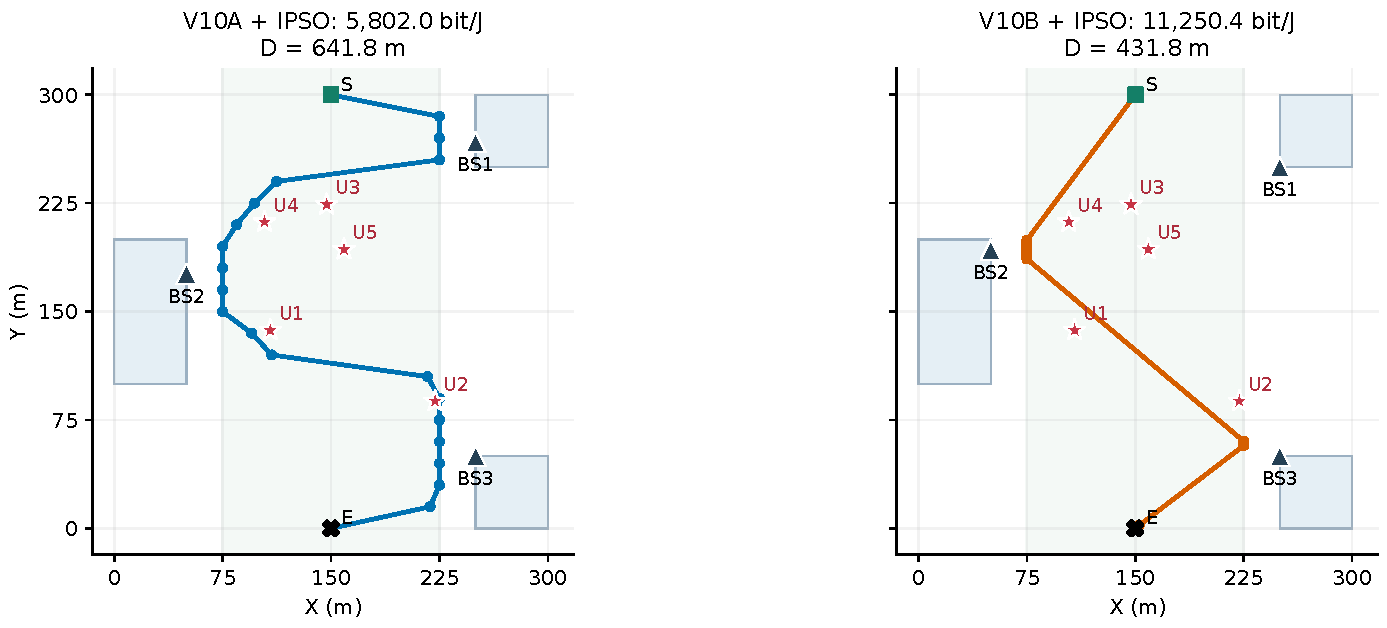
\includegraphics[width=\textwidth,height=4.55cm,keepaspectratio]{trajectory_2026.pdf}
\caption{IPSO, $q=5$ kbit/user/slot, hover 1 s; cả hai nghiệm khả thi. UAV $Z=30$ m. Sao đỏ: user; tam giác: BS; S/E: đầu/cuối; chấm: waypoint; ô xanh nhạt: miền BS. B gom nhiều điểm phục vụ, tăng EE và rút ngắn đường bay.}
\end{figure}
\end{frame}

% 7/10
\begin{frame}{Quỹ đạo và BS tại L=3 Mbit: seed 3486784401}
\begin{figure}\centering
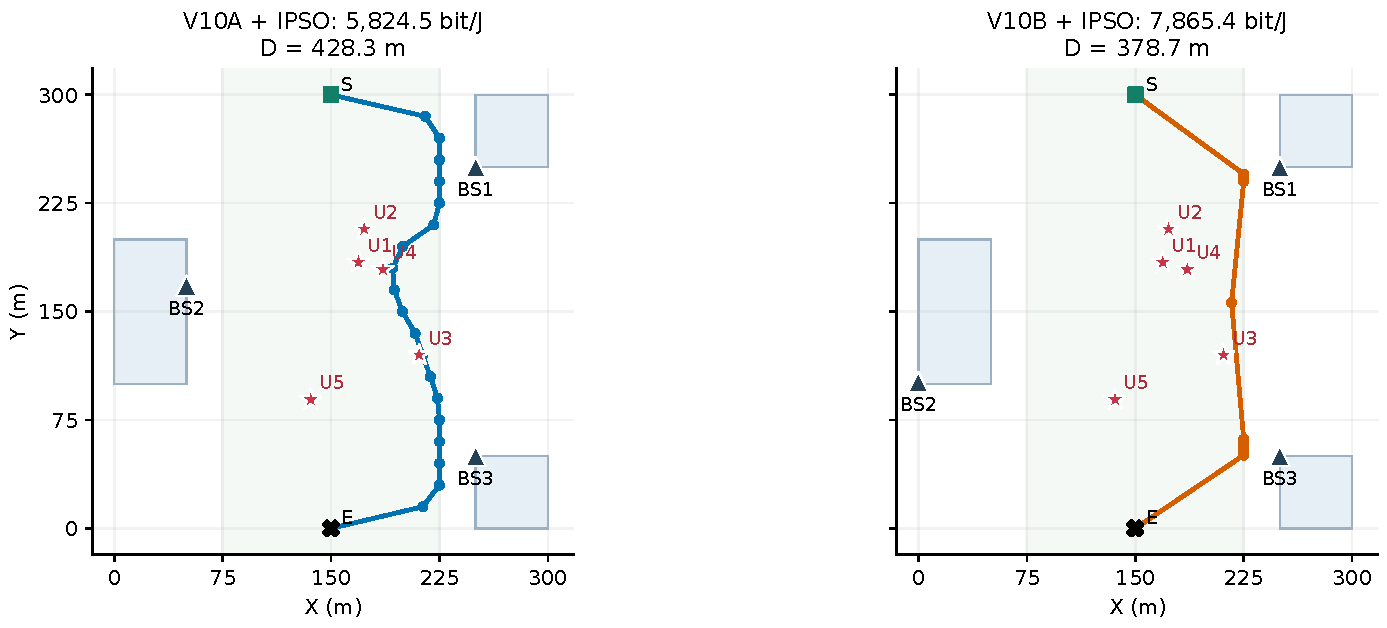
\includegraphics[width=\textwidth,height=4.55cm,keepaspectratio]{trajectory_3486784401.pdf}
\caption{IPSO, $q=5$ kbit/user/slot, hover 1 s; cả hai nghiệm khả thi. UAV $Z=30$ m; BS1/2/3 có độ cao 20/30/25 m. BS2 của B ở $(0,101{,}26,30)$ m, cho thấy vị trí BS phụ thuộc scenario. Tọa độ đọc trực tiếp từ MAT.}
\end{figure}
\end{frame}

% 8/10
\begin{frame}{Tọa độ BS của ba seed tại L=3 Mbit}
\footnotesize\begin{table}
\centering\renewcommand{\arraystretch}{1.03}\setlength{\tabcolsep}{6pt}
\begin{tabular}{lllrr}\toprule
Bản & Seed & Thuật toán & BS1 $(x,y)$ & BS2 $(x,y)$ \\
\midrule
V10A & 2026 & PSO & (250.00, 277.83) & (50.00, 184.39) \\
V10A & 2026 & IPSO & (250.00, 267.19) & (50.00, 176.17) \\
V10A & 608060 & PSO & (250.00, 250.00) & (50.00, 158.45) \\
V10A & 608060 & IPSO & (250.00, 253.13) & (50.00, 157.91) \\
V10A & 3486784401 & PSO & (250.00, 250.00) & (50.00, 200.00) \\
V10A & 3486784401 & IPSO & (250.00, 250.00) & (50.00, 167.98) \\
\midrule
V10B & 2026 & PSO & (250.00, 300.00) & (50.00, 173.91) \\
V10B & 2026 & IPSO & (250.00, 250.00) & (50.00, 192.90) \\
V10B & 608060 & PSO & (250.00, 300.00) & (50.00, 149.58) \\
V10B & 608060 & IPSO & (250.00, 279.99) & (50.00, 150.48) \\
V10B & 3486784401 & PSO & (250.00, 250.00) & (49.83, 100.00) \\
V10B & 3486784401 & IPSO & (250.00, 250.00) & (0.00, 101.26) \\
\bottomrule\end{tabular}
\caption{Giữ $q=5$ kbit/user/slot, hover 1 s; cả 12 nghiệm khả thi. Đơn vị m, làm tròn 0,01 m. Mọi hàng có BS3=$(250,50,25)$ m; độ cao BS1=20 m, BS2=30 m. PSO là Full PSO; CSV đính kèm giữ đủ X/Y/Z.}\end{table}

\end{frame}

% 9/10
\begin{frame}{BS thường chạm biên: có thể thử cố định tọa độ nào?}
\small
\begin{table}\centering
\begin{tabular}{lrrr}\toprule
Ứng viên & Bộ chính $q=5,h=1$ & Mọi bộ $L=3$ & Chỉ nghiệm khả thi\\\midrule
$x_{\rm BS1}=250$ m & 12/12 & 59/60 & 58/59\\
$x_{\rm BS2}=50$ m & 10/12 & 51/60 & 50/59\\
$x_{\rm BS3}=250$ m & 12/12 & 60/60 & 59/59\\
BS3=$(250,50,25)$ m & 12/12 & 50/60 & 49/59\\\bottomrule
\end{tabular}\caption{60 nghiệm Full sau loại trùng: A/B, ba seed, năm bộ $(q,h)$, hai thuật toán. Sai số chạm tọa độ $\leq10^{-3}$ m.}
\end{table}
\begin{block}{Ứng viên kiểm tra trước}
\small Thử cố định $x_{\rm BS3}=250$, rồi $x_{\rm BS1}=250$. Với riêng bộ chính, có thể thử cố định toàn bộ BS3=$(250,50,25)$ m.
\end{block}
\notevi{BS chỉ được dịch X/Y trong khoảng $\pm50$ m quanh vị trí gốc, cắt tại vùng $300\times300$ m. Xu hướng chạm biên chịu ảnh hưởng miền này. Giữ $y_1$, BS2 và $y_3$ linh hoạt khi xét nhiều $q,h$.}
\notevi{Cần chạy lại khi cố định để đo mất EE và QoS. Báo cáo chưa thay đổi BS hoặc kiểm chứng phương án cố định.}
\end{frame}

% 10/10
\begin{frame}{Kết luận và giới hạn của kết quả hiện có}
\small
\begin{itemize}
\item \hi{V10B + IPSO cho EE cao hơn A nhất quán trong campaign.} Trung bình 21 cấu hình: 9.956,75 so với 6.452,96 bit/J; gain ghép cặp 55,79\%.
\item \hi{EE tăng đi kèm dữ liệu tập trung hơn.} Jain trung bình giảm từ 0,749 ở A xuống 0,569 ở B. Cần cân nhắc fairness khi chọn cấu hình.
\item \hi{IPSO có tỷ lệ khả thi cao nhất, nhưng không thắng PSO mọi lần.} Chỉ có ba scenario seed, cùng một seed thuật toán; mutation/polishing làm chi phí đánh giá khác nhau.
\end{itemize}
\vspace{2mm}
\footnotesize\textbf{Tệp đính kèm:} nguồn Beamer, hình vector, EE tổng hợp, tọa độ BS và waypoint UAV. Bảng chi tiết từng seed giữ trong dữ liệu, không thêm phụ lục vào PDF.
\vspace{2mm}
\src{[1] T. Zhang et al., \emph{Trajectory and Power Control for Sustainable UAV-Assisted NOMA-Enabled Backscattering IoT}, Drones 2026, 10, 238. \href{https://doi.org/10.3390/drones10040238}{doi:10.3390/drones10040238}. Dữ liệu: \texttt{campaign\_20261029\_125559}; cấu hình và kết quả cuối từ 54 MAT. Mô hình V10 dùng cruise + hover + RF, chưa tính gia tốc/rẽ/mạch/PA.}
\end{frame}
\end{document}

